% Compile with: pdflatex weekly_progress2.tex (run twice)

\documentclass[10pt,aspectratio=169]{beamer}

\usepackage[utf8]{inputenc}
\usepackage[T1]{fontenc}
\usepackage{lmodern}
\usepackage{amsmath, amssymb}
\usepackage{tikz}
\usepackage{booktabs}
\usepackage[table]{xcolor}
\usepackage{array}
\usepackage{graphicx}

\usetikzlibrary{positioning, shapes.geometric, arrows.meta, backgrounds, fit, calc}

\usetheme{Madrid}
\usecolortheme{seahorse}
\setbeamertemplate{navigation symbols}{}
\setbeamertemplate{caption}[numbered]
\setbeamerfont{frametitle}{size=\large}
\setbeamerfont{title}{size=\Large}

\definecolor{paperA}{RGB}{200,80,80}
\definecolor{paperB}{RGB}{60,100,180}
\definecolor{paperC}{RGB}{130,60,180}
\definecolor{paperD}{RGB}{50,140,80}
\definecolor{boxbg}{RGB}{240,240,250}
\definecolor{frozenbg}{RGB}{220,220,220}
\definecolor{trainedbg}{RGB}{255,235,205}
\colorlet{accent}{paperB}

\tikzstyle{block}  = [rectangle, draw, rounded corners, align=center,
                      minimum height=0.8cm, minimum width=2.2cm, fill=boxbg]
\tikzstyle{frozen} = [block, fill=frozenbg]
\tikzstyle{trained}= [block, fill=trainedbg]
\tikzstyle{arrow}  = [-{Stealth[length=2mm]}, thick]

\title[av\_ib Weekly Progress]{Audio-Visual Information Bottleneck\\
       \normalfont\normalsize Weekly Progress --- Causal Diagnosis, the Best Configuration \& the Fail-Safe Pivot}
\subtitle{}
\author{}
\institute{}
\date{\today}

\begin{document}

\frame{\titlepage}

% =====================================================================
\section{This week}

\begin{frame}{What I did this week}

\begin{block}{Found the best way to bottleneck: frozen LLM + bottleneck only (no LoRA)}
  At matched compression, a bottleneck-only model (no LoRA) beats
  LoRA$+$bottleneck (84\,\% vs 80\,\%) and costs only $\sim$2\,pp vs.\ the
  uncompressed baseline for 2.6$\times$ video compression. The bottleneck is a
  good \emph{lossy filter}.
\end{block}

\begin{block}{But then: \emph{why} does the model ignore audio? --- it's the benchmark}
  Causal per-modality ablation on MUSIC-AVQA: removing audio barely changes the
  model's answer ($+8.3$\,\% NLL, accuracy $65\to62.5$\,\%), and only
  $\sim$0.5\,\% of questions are genuinely audio-visual. The benchmark
  structurally \textbf{cannot} test an AV bottleneck --- so the accuracy numbers
  are the wrong yardstick.
\end{block}

\begin{block}{Tested fail-safety on AVHBench --- and it regressed}
  the model became \textbf{more credulous} (Video-driven Audio Hallucination
  $-8.3$\,pp). A lossy filter is not a safety mechanism. $\Rightarrow$ pivot to
  an explicit \textbf{fail-safe abstention} experiment (SFT vs DPO), now running.
\end{block}

\end{frame}

% =====================================================================
\section{Best configuration}

\begin{frame}{Frozen LLM + bottleneck only is the best way to bottleneck}

\begin{columns}[T]
\begin{column}{0.50\textwidth}
\centering
\scalebox{0.82}{%
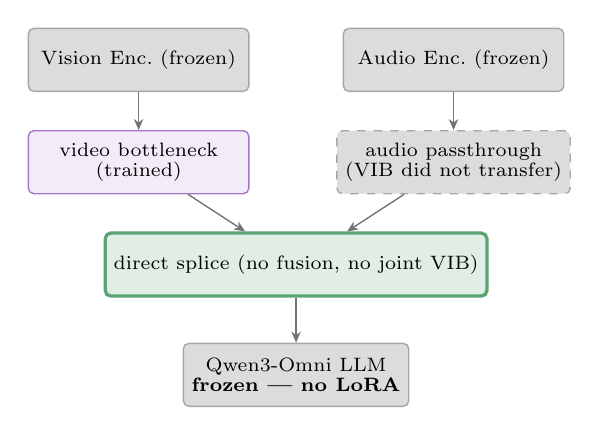
\begin{tikzpicture}[
  font=\scriptsize,
  >={Stealth[length=1.4mm,width=1.2mm]},
  frz/.style={rectangle, rounded corners=2pt, draw=black!35,
              fill=frozenbg, line width=0.5pt, align=center,
              minimum width=28mm, minimum height=8mm, inner sep=3pt},
  trn/.style={rectangle, rounded corners=2pt, draw=paperC!70,
              fill=paperC!10, line width=0.5pt, align=center,
              minimum width=28mm, minimum height=8mm, inner sep=3pt},
  idn/.style={rectangle, rounded corners=2pt, draw=black!35,
              fill=frozenbg, line width=0.5pt, align=center, dashed,
              minimum width=28mm, minimum height=8mm, inner sep=3pt},
  win/.style={rectangle, rounded corners=2pt, draw=paperD!80,
              fill=paperD!15, line width=1.2pt, align=center,
              minimum width=46mm, minimum height=8mm, inner sep=3pt},
  arr/.style={->, line width=0.5pt, draw=black!55}
]
\node[frz] (venc) at (-2.0, 2.8) {Vision Enc.\ (frozen)};
\node[frz] (aenc) at ( 2.0, 2.8) {Audio Enc.\ (frozen)};
\node[trn] (vvib) at (-2.0, 1.5) {video bottleneck\\[-1pt](trained)};
\node[idn] (avib) at ( 2.0, 1.5) {audio passthrough\\[-1pt](VIB did not transfer)};
\node[win] (splice) at (0, 0.2) {direct splice (no fusion, no joint VIB)};
\node[frz] (llm)  at ( 0,  -1.2) {Qwen3-Omni LLM\\[-1pt]\textbf{frozen --- no LoRA}};
\draw[arr] (venc)--(vvib); \draw[arr] (aenc)--(avib);
\draw[arr] (vvib)--(splice);  \draw[arr] (avib)--(splice);
\draw[arr] (splice)--(llm);
\end{tikzpicture}}

\vspace{2pt}
{\footnotesize \textbf{Video-only bottleneck}: only the video VIB trains. We
tried to apply the same bottleneck to audio but couldn't get it to work, so
audio passes through untouched (it was inert anyway).}
\end{column}

\begin{column}{0.47\textwidth}

\begin{block}{Held-out accuracy (150 samples)}
{\footnotesize
\begin{tabular}{l r r}
\toprule
\textbf{Config} & \textbf{Acc.} & \textbf{$\mathrm{KL}_v$} \\
\midrule
LoRA, no bottleneck & 86.0\,\% & 12229 \\
\rowcolor{paperD!12}
\textbf{bottleneck only, no LoRA} & \textbf{84.0\,\%} & \textbf{4776} \\
LoRA $+$ bottleneck & 80.0\,\% & 4710 \\
untrained (vanilla) & 76.7\,\% & 12229 \\
\bottomrule
\end{tabular}}
\end{block}

\begin{block}{What the numbers say}
{\footnotesize
We train $\mathcal L=\text{NLL}+\beta\,\mathrm{KL}_v$ with
$\mathrm{KL}_v=\tfrac12\sum_j(\mu_j^2+\sigma_j^2-1-\log\sigma_j^2)$. This
$\mathrm{KL}_v$ \emph{is} the code's information rate $I(X_v;Z_v)$, so the
acc-vs-$\mathrm{KL}_v$ table is a \textbf{rate--distortion curve}: raising
$\beta$ lowers the rate ($12229\!\to\!4710\!\to\!2301$) and accuracy falls
monotonically. At matched rate, freezing the LLM (84\,\%) beats LoRA$+$bottleneck
(80\,\%); $2.6\times$ compression costs $\sim$2\,pp.\\[3pt]
Audio is \emph{stuck} at $\mathrm{KL}_a\!\approx\!490$: with
$I(X_a;Y\,|\,X_v)\!\approx\!0$ there is no relevance gradient to trade against
its rate, so nothing trains --- we leave audio untouched.}
\end{block}

\end{column}
\end{columns}

\vspace{2pt}
\begin{block}{Puzzle: plain LoRA wins, and the bottleneck \emph{costs} accuracy}
{\footnotesize
The uncompressed LoRA baseline (86\,\%) beats everything, and adding the
bottleneck only lowers accuracy. So is the bottleneck useless? \textbf{Only if
accuracy on this benchmark means what we think it does} --- which is exactly
what we checked next.}
\end{block}

\end{frame}

% =====================================================================
\section{Diagnosis}

\begin{frame}{Hold on --- MUSIC-AVQA cannot test an AV bottleneck}

\begin{block}{The test (40 items, vanilla model)}
{\footnotesize
Delete one modality's tokens and measure how much worse the model predicts the
correct answer ($\Delta$NLL). \textbf{If the answer barely degrades, the model
never needed that modality.}}
\end{block}

\begin{columns}[T]
\begin{column}{0.54\textwidth}
\centering
{\footnotesize
\begin{tabular}{l l r r}
\toprule
\textbf{Delete} & \textbf{Left} & \textbf{$\Delta$NLL} & \textbf{Acc.} \\
\midrule
nothing \emph{(ref.)} & audio+video & --- & 65.0\,\% \\
\rowcolor{paperD!12}
\textbf{audio} & video only & \textbf{$+8.3$\,\%} & 62.5\,\% \\
video & audio only & $+57.5$\,\% & 57.5\,\% \\
both \emph{(zero)} & nothing & $+48.7$\,\% & 65.0\,\% \\
both \emph{(mean)} & nothing & $+29.7$\,\% & 35.0\,\% \\
both \emph{(shuffle)} & nothing & $+6.3$\,\% & 57.5\,\% \\
\bottomrule
\end{tabular}}
\end{column}

\begin{column}{0.44\textwidth}
\begin{block}{What we find}
{\footnotesize
Dropping \textbf{audio} costs almost nothing ($+8.3$\,\% NLL, $-2.5$\,pp
accuracy) --- the model barely uses it. Removing \emph{both} streams still
leaves accuracy at $65$\,\%, and only $\sim$\textbf{0.5\,\%} of questions are
genuinely audio-visual.}
\end{block}
\end{column}
\end{columns}

\vspace{4pt}
\begin{block}{Conclusion --- so the 86\,\% vs 84\,\% was the wrong yardstick}
{\footnotesize
Read as mutual information: drop-audio costs almost nothing
$\Rightarrow I(X_a;Y\,|\,X_v,Q)\!\approx\!0$; drop-\emph{both} still scores
$65$\,\% $\Rightarrow I(X_a,X_v;Y\,|\,Q)\!\ll\!H(Y\,|\,Q)$, i.e.\ the answer is
fixed by the prior on the question. A bottleneck only ever maximises $I(Z;Y)$ ---
but here that is already satisfied without audio-visual evidence, so accuracy
\textbf{cannot validate it}. The real payoff is a controllable rate $+$ a
\textbf{fail-safe} knob. So we pivot the evaluation.}
\end{block}

\end{frame}

% =====================================================================
\begin{frame}{Why MUSIC-AVQA \emph{invites} prior-based reasoning}

\begin{columns}[T]
\begin{column}{0.50\textwidth}
\begin{block}{What the benchmark is}
{\footnotesize
$\sim$9.3k videos of \textbf{musical-instrument performances} (22 instruments)
with $\sim$45k QA pairs generated from $\sim$33 \textbf{question templates}
(``Is the \texttt{<instr>} playing?'', ``How many instruments are sounding?'',
``Which instrument starts first?''). Answers come from a \textbf{small closed
vocabulary}: yes/no, small counts, instrument names.}
\end{block}

\begin{block}{Three structural shortcuts}
{\footnotesize
\begin{enumerate}\setlength\itemsep{2pt}
  \item \textbf{Templates leak the answer type}: ``how many\ldots'' is almost
        always a small count; the per-template answer distribution is highly
        skewed, so the modal answer alone scores well.
  \item \textbf{The domain is narrow}: every clip is a performance, so
        ``Is the instrument playing?'' defaults to \emph{yes} ---
        instruments in performance videos are usually playing.
  \item \textbf{The question names the entities}: when the prompt already says
        ``the violin,'' identifying the instrument from pixels or sound is
        unnecessary.
\end{enumerate}}
\end{block}
\end{column}

\begin{column}{0.46\textwidth}
\begin{block}{The information-theoretic reading}
{\footnotesize
A model trained with cross-entropy fits $p(y\,|\,Q,X_a,X_v)$. If the
template+domain prior $p(y\,|\,Q)$ already concentrates on the right answer,
then $I(X_a,X_v;Y\,|\,Q)\!\approx\!0$ and the loss is minimised by
\textbf{ignoring the evidence}. The model is not failing --- it is doing
exactly what the objective rewards on this data.}
\end{block}

\begin{block}{And our measurements confirm it}
{\footnotesize
Delete \emph{both} modalities $\Rightarrow$ accuracy stays at 65\,\%
(the prior alone); delete audio $\Rightarrow$ $+8.3$\,\% NLL only.
Only $\sim$0.5\,\% of sampled questions \emph{require} combining audio and
video. The benchmark trains and rewards a \textbf{language-prior policy}.}
\end{block}
\end{column}
\end{columns}

\end{frame}

% =====================================================================
\begin{frame}{Example questions --- templated vs.\ open-domain AVQA}

\begin{columns}[T]
\begin{column}{0.48\textwidth}
\begin{block}{MUSIC-AVQA (templated, narrow domain)}
{\footnotesize
\begin{itemize}\setlength\itemsep{2pt}
  \item ``Is the \emph{guitar} in the video always playing?'' \hfill
        \textcolor{paperA}{prior: \emph{yes}}
  \item ``How many instruments are sounding in the video?'' \hfill
        \textcolor{paperA}{prior: \emph{one/two}}
  \item ``Which is the musical instrument that sounds at the same time as the
        \emph{piano}?'' \hfill \textcolor{paperA}{entities named in prompt}
  \item ``Is there a \emph{voiceover}?'' \hfill \textcolor{paperA}{prior: \emph{no}}
\end{itemize}
Closed answer set, skewed per-template distributions $\Rightarrow$ guessable
without looking or listening.}
\end{block}
\end{column}

\begin{column}{0.48\textwidth}
\begin{block}{AVQA / VGGSound-based (open domain)}
{\footnotesize
\begin{itemize}\setlength\itemsep{2pt}
  \item ``What is making the sound in the background?'' \hfill
        \textcolor{paperD}{must \emph{listen}}
  \item ``Why did the crowd suddenly cheer?'' \hfill
        \textcolor{paperD}{must \emph{look + listen}}
  \item ``What happened after the glass broke?'' \hfill
        \textcolor{paperD}{audio event grounds the answer}
  \item ``Where is the barking dog?'' \hfill
        \textcolor{paperD}{sound source must be localised in the frame}
\end{itemize}
Everyday scenes ($\sim$57k VGGSound clips), free-form events: the question text
alone does not determine the answer.}
\end{block}
\end{column}
\end{columns}

\vspace{4pt}
\begin{block}{Consequence for us}
{\footnotesize
The pathology is a property of \textbf{templated, narrow-domain} benchmarks, not
of AVQA in general. Candidate next testbeds where
$I(X_a,X_v;Y\,|\,Q)$ is genuinely large: VGGSound-based AVQA and our own
corruption-based fail-safe protocol (which manufactures evidence-dependence by
construction).}
\end{block}

\end{frame}

% =====================================================================
\section{AVHBench}

\begin{frame}{AVHBench --- the filter is not a fail-safe}

\begin{columns}[T]
\begin{column}{0.42\textwidth}

\begin{block}{The test}
{\footnotesize
A good safety mechanism should \emph{refuse} (or hedge) when the evidence
behind an answer is corrupted. We ran the bottleneck-only model vs vanilla on
AVHBench (200 items) with focus on Video-driven Audio Hallucination --- the task
where the model is asked to confirm audio content that has been replaced.}
\end{block}

\begin{block}{Result}
{\footnotesize
The bottleneck model $\approx$ vanilla overall, but on the hallucination task it
got \textbf{worse}: it says ``yes'' to mismatched audio \emph{more} often.
The bottleneck removed information without making the model aware that
information was missing.}
\end{block}

\end{column}

\begin{column}{0.55\textwidth}
\scriptsize
\begin{tabular}{l r r r}
\toprule
\textbf{Model} & \textbf{Overall} & \textbf{yes\%} & \textbf{$\Delta$} \\
\midrule
Vanilla   & 69.5\% & 38\% & --- \\
\rowcolor{paperA!8}
Bottleneck only & 67.5\% & 57\% & $-2.0$\,pp \\
\bottomrule
\end{tabular}

\vspace{6pt}
\begin{tabular}{l r r r}
\toprule
\textbf{Video-driven Audio Hall.} & \textbf{Base} & \textbf{Bttlnk} & \textbf{$\Delta$} \\
\midrule
\rowcolor{paperA!10}
Accuracy & 69.8\% & 61.5\% & $-8.3$\,pp \\
yes-rate & 38\% & 57\% & $+19$\,pp \\
\bottomrule
\end{tabular}

\vspace{8pt}
\begin{alertblock}{What is happening}
{\footnotesize
Caution would require the posterior to \emph{flatten}
when evidence is weak ($\max_y p(y|x)\!\downarrow$). Instead, discarding evidence
makes the answer regress toward the unconditional prior
$p(y)$ --- and here the credulous default is ``yes,'' so the yes-rate climbs
$38\!\to\!57$\,\%. \textbf{Compression moves the model toward its prior, not
toward abstention.} Fail-safety must therefore be \emph{trained}, not assumed.}
\end{alertblock}
\end{column}
\end{columns}

\end{frame}

% =====================================================================
% helper: map data coords to tikz cm inside a fixed plot box
% Plot box: x in [0,14000]->0..4cm, y in [72,90]->0..3.6cm

\section{Graphs}

\begin{frame}{The week in two graphs}

\begin{columns}[T]

% ---- plot 1: rate-distortion ----
\begin{column}{0.48\textwidth}
\centering
{\scriptsize\textbf{Rate--distortion: accuracy vs.\ $\mathrm{KL}_v$}}\\[3pt]
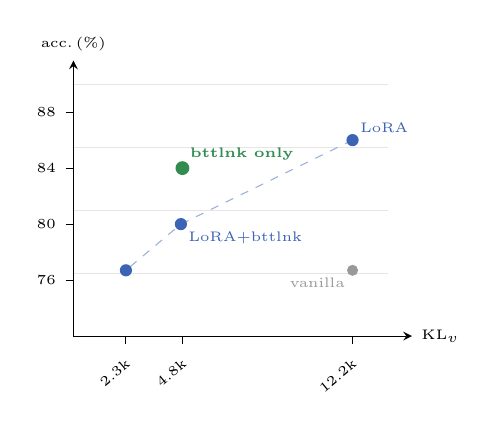
\begin{tikzpicture}[font=\tiny, >=stealth]
% axes: box 4cm wide x 3.2cm tall
% x: 0..14000 -> 0..4, y: 72..90 -> 0..3.2
\def\xsc{0.0002857} % 4/14000
\def\ysc{0.17778}   % 3.2/18
\def\yoff{72}
\pgfmathsetmacro{\Ax}{12229*\xsc} \pgfmathsetmacro{\Ay}{(86.0-\yoff)*\ysc}
\pgfmathsetmacro{\Bx}{4710*\xsc}  \pgfmathsetmacro{\By}{(80.0-\yoff)*\ysc}
\pgfmathsetmacro{\Cx}{2301*\xsc}  \pgfmathsetmacro{\Cy}{(76.7-\yoff)*\ysc}
\pgfmathsetmacro{\Dx}{4776*\xsc}  \pgfmathsetmacro{\Dy}{(84.0-\yoff)*\ysc}
\pgfmathsetmacro{\Ex}{12229*\xsc} \pgfmathsetmacro{\Ey}{(76.7-\yoff)*\ysc}
% grid
\draw[black!10] (0,0.8) -- (4,0.8);
\draw[black!10] (0,1.6) -- (4,1.6);
\draw[black!10] (0,2.4) -- (4,2.4);
\draw[black!10] (0,3.2) -- (4,3.2);
% axes
\draw[->] (0,0) -- (4.3,0) node[right] {$\mathrm{KL}_v$};
\draw[->] (0,0) -- (0,3.5) node[above] {acc.\,(\%)};
% y ticks
\foreach \yv/\yl in {76/76,80/80,84/84,88/88}{
  \pgfmathsetmacro{\yp}{(\yv-\yoff)*\ysc}
  \draw (0,\yp) -- (-0.1,\yp) node[left] {\yl};
}
% x ticks
\foreach \xv/\xl in {2301/2.3k,4776/4.8k,12229/12.2k}{
  \pgfmathsetmacro{\xp}{\xv*\xsc}
  \draw (\xp,0) -- (\xp,-0.1) node[below,rotate=40,anchor=north east] {\xl};
}
% LoRA trend line
\draw[paperB!50, dashed] (\Ax,\Ay) -- (\Bx,\By) -- (\Cx,\Cy);
% points
\fill[paperB]  (\Ax,\Ay) circle(2.2pt) node[above right=-1pt] {LoRA};
\fill[paperB]  (\Bx,\By) circle(2.2pt) node[below right=-1pt] {LoRA$+$bttlnk};
\fill[paperB]  (\Cx,\Cy) circle(2.2pt);
\fill[paperD]  (\Dx,\Dy) circle(2.5pt) node[above right=-1pt] {\textbf{bttlnk only}};
\fill[black!40](\Ex,\Ey) circle(2.0pt) node[below left=-1pt] {vanilla};
\end{tikzpicture}\\[2pt]
{\tiny At matched rate, the frozen-LLM point (green) sits 4\,pp above LoRA$+$bottleneck.}
\end{column}

% ---- plot 2: ΔNLL bar chart ----
\begin{column}{0.48\textwidth}
\centering
{\scriptsize\textbf{Ablation: $\Delta$NLL when evidence is deleted}}\\[3pt]
\begin{tikzpicture}[font=\tiny]
% 5 bars, max 65, box 4cm x 3.2cm
% bars at x = 0.3, 1.1, 1.9, 2.7, 3.5  width=0.5
\def\ys{0.04923} % 3.2/65
\draw[->] (0,0) -- (0,3.5) node[above] {$\Delta$NLL (\%)};
\draw[->] (0,0) -- (4.4,0);
% y ticks
\foreach \yv in {10,20,30,40,50,60}{
  \pgfmathsetmacro{\yp}{\yv*\ys}
  \draw (0,\yp)--(-0.1,\yp) node[left]{\yv};
}
% bars: (x-center, value, label)
\foreach \xc/\val/\lbl in {
  0.35/8.3/audio,
  1.10/6.3/shuffle,
  1.85/29.7/mean,
  2.60/48.7/zero,
  3.35/57.5/video}{
  \pgfmathsetmacro{\ht}{\val*\ys}
  \pgfmathsetmacro{\xlo}{\xc-0.25}
  \pgfmathsetmacro{\xhi}{\xc+0.25}
  \fill[paperB!50,draw=paperB] (\xlo,0) rectangle (\xhi,\ht);
  \node[above,rotate=45,anchor=south west,font=\tiny] at (\xc,\ht) {\val\,\%};
  \node[below,rotate=45,anchor=north east,font=\tiny] at (\xc,-0.05) {\lbl};
}
% highlight audio bar
\draw[paperA, thick] (0.10,0) rectangle (0.60,{8.3*\ys});
\end{tikzpicture}\\[2pt]
{\tiny Removing audio ($+8.3$\,\%) $\approx$ shuffling everything ($+6.3$\,\%). Only video matters.}
\end{column}

\end{columns}

\end{frame}

% =====================================================================
\section{Fail-safe pivot}

\begin{frame}{The pivot --- fail-safe abstention (risk--coverage)}

\begin{columns}[T]
\begin{column}{0.50\textwidth}

\begin{block}{Idea --- a gate $g$ on top of the predictor $f$}
{\footnotesize
Answer $f(x)$ when the gate $g(x)\!=\!1$, else say \textbf{``I can't tell.''}
Score by \textbf{risk--coverage}:
\[
\varphi=\mathbb E[g(x)],\qquad
R=\frac{\mathbb E[\ell(f(x),y)\,g(x)]}{\varphi}.
\]
The optimal gate answers only on high confidence:
$g(x)=\mathbf 1[\max_y p(y|x)\!\ge\!\theta]$. A fail-safe model drops coverage
$\varphi$ under corruption while holding risk $R$ low.}
\end{block}

\begin{block}{Supervision (empirical label miner)}
{\footnotesize
Mined MUSIC-AVQA for items the model gets right under clean evidence but wrong
when video is removed. Yield: \textbf{2815 preference pairs}\\
(abstain 570, capability-anchor 2017, negative-control 228).}
\end{block}

\end{column}

\begin{column}{0.47\textwidth}

\begin{block}{Corruption taxonomy}
{\footnotesize
\begin{tabular}{l p{3.2cm}}
\toprule
\textbf{Group} & \textbf{Modes} \\
\midrule
Train (seen) & \texttt{vid\_zero}, \texttt{vid\_mean} \\
\rowcolor{paperD!12}
Held-out & \texttt{vid\_noise}, \texttt{vid\_scale} \\
Neg.\ control & \texttt{aud\_zero}, \texttt{aud\_mean} \\
\bottomrule
\end{tabular}}
\end{block}

\begin{block}{The decisive test}
{\footnotesize
Generalisation to \textbf{held-out} corruptions never seen in training.
Negative control checks the model does \emph{not} abstain when only the inert
(audio) modality is degraded --- i.e.\ it preserves coverage.}
\end{block}

\end{column}
\end{columns}

\end{frame}

% =====================================================================
\section{SFT vs DPO}

\begin{frame}{SFT vs DPO --- six conditions, head-to-head}

\begin{columns}[T]
\begin{column}{0.48\textwidth}

\begin{block}{Two losses, same data}
{\footnotesize
\textbf{SFT} just minimises NLL of the preferred response:
$\mathcal L_{\text{SFT}}=-\log\pi_\theta(y_w|x)$ --- absolute, no leash to the
base model. \textbf{DPO} optimises the \emph{margin} under a KL leash to the
frozen reference $\pi_{\text{ref}}$:
\[
\mathcal L_{\text{DPO}}=-\log\sigma\!\Big(\beta\big[\log\tfrac{\pi_\theta(y_w|x)}{\pi_{\text{ref}}(y_w|x)}-\log\tfrac{\pi_\theta(y_l|x)}{\pi_{\text{ref}}(y_l|x)}\big]\Big).
\]
The $\pi_{\text{ref}}$ term is why DPO can suppress the credulous ``yes''
\emph{without} drifting from the base model's capability --- the failure mode SFT
risks.}
\end{block}

\begin{block}{Preference pairs (same for both losses)}
{\footnotesize
\begin{tabular}{l p{1.5cm} p{1.5cm}}
\toprule
\textbf{Kind} & \textbf{chosen} & \textbf{rejected} \\
\midrule
abstain (video removed) & ``I can't tell'' & gold \\
anchor (intact) & gold & ``I can't tell'' \\
neg-ctrl (audio only) & gold & ``I can't tell'' \\
\bottomrule
\end{tabular}}
\end{block}

\end{column}

\begin{column}{0.48\textwidth}

\begin{block}{Conditions}
{\footnotesize
\begin{tabular}{l p{3.7cm}}
\toprule
\textbf{LoRA only} & LoRA, no bottleneck \\
\rowcolor{paperC!8}
\textbf{Bottleneck only} & frozen LLM, no LoRA \\
\textbf{Bottleneck + LoRA} & both trained \\
\bottomrule
\end{tabular}
\\[3pt]
$\times$ \{SFT, DPO\} $=$ 6 runs, evaluated by risk--coverage on the same
held-out set.}
\end{block}

\begin{block}{Status (on cluster, 8$\times$H200)}
{\footnotesize
Miner + Stage-0 free probe: \textbf{done}. SFT/DPO training: \textbf{running}
(debugged through path + OOM fixes; model sharded across all GPUs).
Eval chained to fire on completion.}
\end{block}

\end{column}
\end{columns}

\end{frame}

% =====================================================================
\section{Open issue}

\begin{frame}{Open issue --- where the corruption is injected}

\begin{columns}[T]
\begin{column}{0.52\textwidth}

\begin{block}{The problem --- a data-processing argument}
{\footnotesize
The signal path is $X_v\!\to\!Z_v\!\to\!\hat Y$. Corruption $c$ is currently
applied to the code $Z_v$ (downstream of the VIB):
\begin{itemize}\setlength\itemsep{2pt}
  \item \textbf{LoRA conditions} (adapters \emph{below} $c$): the LLM sees the
        degraded tokens, so $\partial\mathcal L/\partial\theta_{\text{LoRA}}\!\neq\!0$.
        \textcolor{paperD}{Trains fine.}
  \item \textbf{Bottleneck-only} (frozen LLM): $Z_v$ is computed \emph{before}
        $c$, so the VIB never sees it $\Rightarrow
        \partial\mathcal L/\partial\theta_{\text{VIB}}\!=\!0$ on \texttt{vid\_zero}
        (the $\text{gn}\!=\!0$ we logged). \textcolor{paperA}{Structurally cannot fail-safe.}
\end{itemize}}
\end{block}

\end{column}

\begin{column}{0.46\textwidth}

\begin{block}{The fix (pending decision)}
{\footnotesize
To fairly test the bottleneck hypothesis (degraded evidence in
$\Rightarrow$ low-information code out $\Rightarrow$ frozen LLM abstains),
the corruption must be injected \textbf{upstream of the VIB}, on the encoder
output. This requires re-mining labels with upstream corruption.\\[4pt]
\textbf{Note:} the LoRA conditions' results from the current run remain valid either way.}
\end{block}

\end{column}
\end{columns}

\begin{center}
\scalebox{0.9}{%
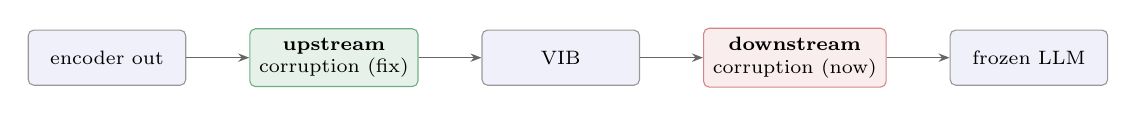
\begin{tikzpicture}[font=\scriptsize, >={Stealth[length=1.4mm]},
  b/.style={rectangle, rounded corners=2pt, draw=black!40, fill=boxbg,
            minimum height=7mm, minimum width=20mm, align=center},
  bad/.style={b, draw=paperA!70, fill=paperA!10},
  good/.style={b, draw=paperD!70, fill=paperD!12},
  arr/.style={->, line width=0.6pt, draw=black!60}]
\node[b] (enc) {encoder out};
\node[good, right=8mm of enc] (up) {\textbf{upstream}\\corruption (fix)};
\node[b, right=8mm of up] (vib) {VIB};
\node[bad, right=8mm of vib] (down) {\textbf{downstream}\\corruption (now)};
\node[b, right=8mm of down] (llm) {frozen LLM};
\draw[arr] (enc)--(up); \draw[arr] (up)--(vib); \draw[arr] (vib)--(down); \draw[arr] (down)--(llm);
\end{tikzpicture}}
\end{center}

\end{frame}

% =====================================================================
\section{Next steps}

\begin{frame}{Next steps}

\begin{block}{1.\ Decide corruption placement, then finish the 6-way comparison}
  Resolve the upstream-vs-downstream question; relabel if needed. Then read
  risk--coverage on held-out corruptions: does the bottleneck generalise
  fail-safety better than LoRA alone?
\end{block}

\begin{block}{2.\ Transfer the winner to AVHBench}
  Run the best abstention model on the Video-driven Audio Hallucination task
  (the $-8.3$\,pp regression) --- the real out-of-distribution test of fail-safety.
\end{block}

\begin{block}{3.\ Decide the deliverable}
  \begin{itemize}\setlength\itemsep{2pt}
    \item bottleneck $\gg$ LoRA-alone on held-out $\Rightarrow$ bottleneck buys fail-safe generalisation. \textbf{Ship the method.}
    \item bottleneck $\approx$ LoRA-alone $\Rightarrow$ bottleneck not needed; DPO alone fixes it. \textbf{Ship the benchmark diagnosis + simpler remedy.}
    \item all $\approx$ baseline $\Rightarrow$ \textbf{ship the benchmark-diagnosis finding} (the evaluation pathology) alone.
  \end{itemize}
\end{block}

\end{frame}

\end{document}
